% !TEX program = tectonic
% Corrected version of "Sequential Assembly of Biological Agency"
% for upload to SSRN abstract 6593781.
%
% This document does NOT rewrite the original paper. It prepends a
% correction notice and stamps every page of the original, which is
% included unmodified from genesis_paper_farina_2026.pdf (v5.3, the
% version currently posted). The original text must stay readable:
% the companion methods paper argues its defects are only legible
% against it.
%
% Build: tectonic genesis_paper_v6_corrected.tex
\documentclass[11pt,letterpaper]{article}

\usepackage[letterpaper,margin=1in,top=1.15in]{geometry}
\usepackage[T1]{fontenc}
\usepackage{lmodern}
\usepackage[utf8]{inputenc}
\usepackage{microtype}
\usepackage{textcomp}
\usepackage{amsmath,amssymb}
\usepackage{enumitem}
\usepackage{xcolor}
\definecolor{warn}{rgb}{0.62,0.11,0.06}
\definecolor{rule}{rgb}{0.75,0.75,0.75}

\usepackage[colorlinks=true,linkcolor=black,urlcolor=warn,
            breaklinks=true]{hyperref}
\usepackage{pdfpages}
\usepackage{fancyhdr}
\usepackage{setspace}
\onehalfspacing
\setlength{\parskip}{5pt}
\setlength{\parindent}{0pt}
\setlist{itemsep=3pt,topsep=5pt,leftmargin=1.4em}

% Stamp applied to every page of the included original.
\fancypagestyle{stamp}{%
  \fancyhf{}%
  \renewcommand{\headrulewidth}{0.8pt}%
  \renewcommand{\headrule}{\color{warn}\hrule height 0.8pt}%
  \setlength{\headheight}{16pt}%
  \fancyhead[C]{\footnotesize\color{warn}\bfseries
    CENTRAL RESULT WITHDRAWN --- see correction at front}%
}
\fancypagestyle{front}{%
  \fancyhf{}%
  \renewcommand{\headrulewidth}{0pt}%
  \fancyfoot[C]{\small\thepage}%
}
\pagestyle{front}
\pagenumbering{roman}

\begin{document}

% ── Banner page ──────────────────────────────────────────────────────
\thispagestyle{front}
\vspace*{0.4in}
{\color{warn}\hrule height 2.5pt}
\vspace{10pt}
{\Large\bfseries\color{warn} CORRECTION AND PARTIAL WITHDRAWAL}

\vspace{4pt}
{\large\bfseries Sequential Assembly of Biological Agency}

\vspace{2pt}
SSRN abstract 6593781 \textperiodcentered\ Micka\"el Farina
\vspace{8pt}
{\color{warn}\hrule height 2.5pt}

\vspace{16pt}
\textbf{The central result of the paper that follows is withdrawn.}
Division regularity was reported to precede spatial organization in
1{,}845 of 1{,}845 runs. That result was produced by measurement
artifacts in my own code, not by the dynamics it was attributed to.
Eight defects are documented below, each sufficient on its own to
produce the reported figure.

The paper is reproduced unaltered after this notice rather than
replaced. Its text and data are the evidence for the correction, and
removing them would make the defects harder to check rather than
easier.

\vspace{10pt}
\textbf{Corrected figure.} Measured without the faulty gate, the
ordering holds in approximately 1\,\% of runs.

\vspace{10pt}
\textbf{This correction was found by re-analysis of my own published
code and data.} The repository was public throughout, and the decisive
evidence was already inside the paper's own data files on the day of
posting.

\vspace{14pt}
{\color{rule}\hrule height 0.5pt}
\vspace{6pt}
{\small
Full audit, all experiment scripts and raw outputs:
\url{https://github.com/AVADSA25/genesis-engine} ---
directory \texttt{paper/v6\_supplement/}.

A companion methods paper, \emph{The Detector Was the Result: Eight
Measurement Artifacts, and a Question That Cannot Be Asked This Way},
documents the audit in full, including the errors made while
performing it.

\vspace{4pt}
Correction dated 3 August 2026.
}

\clearpage

% ── Correction notice ────────────────────────────────────────────────
{\large\bfseries Correction notice}

\vspace{2pt}
{\small SSRN abstract 6593781 \textperiodcentered\ 3 August 2026
\textperiodcentered\ Farina}
\vspace{4pt}
{\color{rule}\hrule height 0.5pt}

I withdraw this paper's central result. Re-analysis of my own code and
data shows the reported Clock\,$\rightarrow$\,Map ordering was produced
by measurement artifacts, not the dynamics it was attributed to.

\textbf{Withdrawn:} that division regularity (Clock) preceded spatial
organization (Map) in 1{,}845/1{,}845 runs (100\,\%), binomial
$p = 8.01 \times 10^{-146}$.

\textbf{Eight defects.}

\begin{enumerate}
\item \textbf{The detector could not fail.} \texttt{detect\_phase()}
  latches Map only if Clock latched strictly earlier, so 100\,\% was the
  only reachable outcome; both $p$-values test unreachable nulls.
\item \textbf{The delay is the sampling interval.} Median 50 ticks at
  50-tick sampling; exactly 1 at 1-tick sampling (91 of the 97 re-run
  seeds in which both predicates latched, 93.8\,\%; 3 of 100 never
  latched Map).
\item \textbf{The Clock latch is a definedness floor.} CV is undefined
  until a cell completes four divisions; the tick it becomes computable
  coincides exactly with the reported latch --- 4200 vs 4200 in 1D
  ($n = 500$) and 4900 vs 4900 in 2D ($n = 200$), medians over the full
  archive. A later experiment showed this is only half an error: the
  \emph{specific} four-division floor is mine, but a floor of order
  several division periods is \textbf{physical} --- measuring the
  regularity of a process whose period is $\sim$2{,}540 ticks requires
  observing several of those periods, while the spatial metric is
  defined by $\sim$150 ticks. Measured: such a metric needs $\sim$9
  periods before it tracks regularity at all. See below.
\item \textbf{The mean delay is three runs.} $243 \pm 2{,}319$ ticks is
  carried by seeds 171, 294, 361 (69.0\,\% of delay mass); excluding
  them, 75.7. \texttt{paper\_data.json} already held
  \texttt{median = 50.0} beside the mean.
\item \textbf{The denominator double-counts.} In a one-at-a-time
  ablation the baseline is genuinely shared across parameter groups, and
  printing it in all four rows is standard. The error was summing all
  twelve rows: 1{,}845 $\rightarrow$ \textbf{1{,}554} distinct runs.
\item \textbf{The effect sizes are invalid three ways.} Hedges' $g$ uses
  \texttt{final\_pop} grouped by stability $S$, which multiplies uptake,
  efficiency and maintenance --- so $g$ measures my own coupling
  constants. In 2D the comparison is 198 vs \textbf{2} runs, none
  between thresholds. And the repository's ``combined'' $g = 6.34$ is
  exactly $(9.41 + 3.27)/2$ --- the arithmetic mean of two effect sizes,
  which is not a valid pooling under any convention, one of whose inputs
  has $n = 2$. \S4.3 explained the lower 2D $g$ as ``more spatial
  degrees of freedom'': a physical story invented for an artifact.
\item \textbf{Gate dependence is systematic.} Nine of 19 reported
  quantities depend on detector outputs, and a tenth indirectly.
  Phase-D rates (90\,\%/79\,\%) are withdrawn; only the direction
  survives, and only because two confounds predict the opposite sign.
  \textbf{All four \S5.3 results are withdrawn or demoted --- \S5.3 does
  not survive as physics;} two remain as arithmetic with their causal
  readings withdrawn.
\item \textbf{$\rho(T_{\mathrm{div}}, S) = +0.43$ has the wrong sign.}
  Within each lipid condition it is $-0.60$ to $-0.75$. Pooling reverses
  it: a Simpson's paradox.
\end{enumerate}

\textbf{Corrected figure.} Without the gate, Clock precedes Map in
\textbf{$\approx$1\,\%} of runs ($1/97 = 1.0$\,\% by 1-tick resample;
0.7\,\% by threshold grid, $n = 150$; 0.0\,\% in 2D across all nine
cells).

\textbf{The inverse is also unestablished.} The Map-first signal is
partly the same definedness floor; this model cannot adjudicate the
ordering either way.

\textbf{The corrected measurement was itself validated.} Planting a
known ordering in the physics (280 runs), the ungated method recovered
it: $\rho = +0.96$ between planted and measured, with Clock-first moving
from 2.6\,\% to 100\,\% as the plant crossed the natural Clock time. The
$\approx$1\,\% figure is a real measurement, not a blind instrument.

\textbf{The hypothesis was then tested directly} --- 1{,}350 runs with
regularity imposed as a control variable, no detector or CV estimator in
the path. The association ran opposite to prediction and survived three
of four pre-registered confound checks, including a matched-interval
control that excludes the obvious alternative. It failed the fourth:
barely-dividing cells rise from 44.0\,\% to 56.2\,\% across the range
(threshold 10 pp). It can therefore be \textbf{neither confirmed nor
refuted} by that experiment.

\textbf{The original question is malformed as posed.} Asking which
metric crosses its threshold first compares a slow periodic process
(division regularity, period $\sim$2{,}540 ticks, requiring several
periods to measure at all) against a fast field process (spatial
correlation, $\sim$40 ticks, measurable by $\sim$150). An attempt to
build a Clock metric with no definedness floor failed twice over. A
buffer sweep (four spans, 40 seeds each) shows the replacement does not
track division regularity at all until its history spans $\sim$9 periods
($\rho = -0.46$, $p = 0.003$ on 40 held-out seeds; shorter spans are
indistinguishable from zero and one has the wrong sign). Because the
metric becomes defined exactly when its buffer fills, the earliest a
\emph{valid} Clock reading can exist is $\sim$24{,}000 ticks --- against
a spatial metric defined by $\sim$150, a factor of 160. This is a
time--frequency constraint, not an implementation choice, and no
simulation redesign removes it. Ordering claims of this kind must be
tested by \textbf{intervention}, which is what the imposed-regularity
experiment above did.

\textbf{Also withdrawn:} the Damk\"ohler framing ($\tau_{\text{pattern}}$
was the sampling interval) and the 2D back-reaction ($p = 0.427$). A
v5.1c figure of ``roughly 4\,\%'' should have read 22.8\,\% --- moot, as
the result is withdrawn.

\textbf{What stands:} \S5.2's generalization argument; the 1D
$\Delta$-CV ($-0.222$) and Phase-E differential ($+0.147$), as
arithmetic only; the timescale anchor (15.8--38.3 min, bracketing
\emph{E.\ coli}, fixed a priori); extinction under forced fast division
(32.4\,\% at $T = 200$, zero at $T \geq 1600$; 27.3\,\% at
$\mathrm{CV} = 0$ vs $\leq$4\,\% at $\mathrm{CV} \geq 0.1$) ---
\textbf{both confined to imposed periods $\leq$800, which this model
treats as unphysical; at sustainable rates extinction is zero at every
CV}; and \textbf{one} lipid-supply result confirmed by two measures ---
higher supply $\rightarrow$ lower pattern stability, seen as final $S$
$0.823 \rightarrow 0.644$ and restated in thresholded form by Phase-D
attainment. The \textbf{mechanism is not identified}: an earlier draft
of this note asserted the effect runs \emph{through} faster division,
but within every lipid stratum the correlation between division period
and stability is strongly negative ($-0.60$ to $-0.75$), the opposite of
what that mechanism predicts. Attributing a between-condition
correlation to a plausible mechanism is the same error as defect 6.
These are not three findings; $\rho$ was the third and it is withdrawn.

\textbf{Two cross-validations this paper relied on can no longer be
checked.} No source code survives for the companion Vesicle Division or
Engine studies, so neither the $\mathrm{CV} = 0.06$ agreement cited in
\S4.1 --- offered there as ``an independent validation that our Clock
mechanism captures the same physics as the standalone model'' --- nor
the $g = 4.07$ comparison in the Table~1 caption can be verified. Both
were presented as external corroboration; neither is now checkable.
Additionally, the Vesicle results file has no CV column, so its
published figure cannot be traced even from the data that does survive,
and $g = 4.07$ cannot be checked for the same circularity found here. Genesis Engine published its code. That is the only reason these
eight defects were findable, and correctable, at all.

Found by my own re-analysis; the repository was public throughout and
the evidence sat in the paper's own data files. Full audit:
\texttt{paper/v6\_supplement/}. The audit is ongoing --- further
findings will be recorded in the repository, not issued as further
retractions.

\clearpage

{\large\bfseries The paper as originally published}

\vspace{4pt}
{\color{rule}\hrule height 0.5pt}
\vspace{8pt}

What follows is version 5.3, reproduced without alteration, as posted.
Every page carries a header marking the withdrawal. Read \S4.2, \S4.3
and \S5.3 against defects 1--8 above; those are the sections the
correction bears on most directly.

\clearpage
\pagenumbering{arabic}
% Scaled and nudged down so the withdrawal stamp occupies a clean band
% above the original's own running header rather than overprinting it.
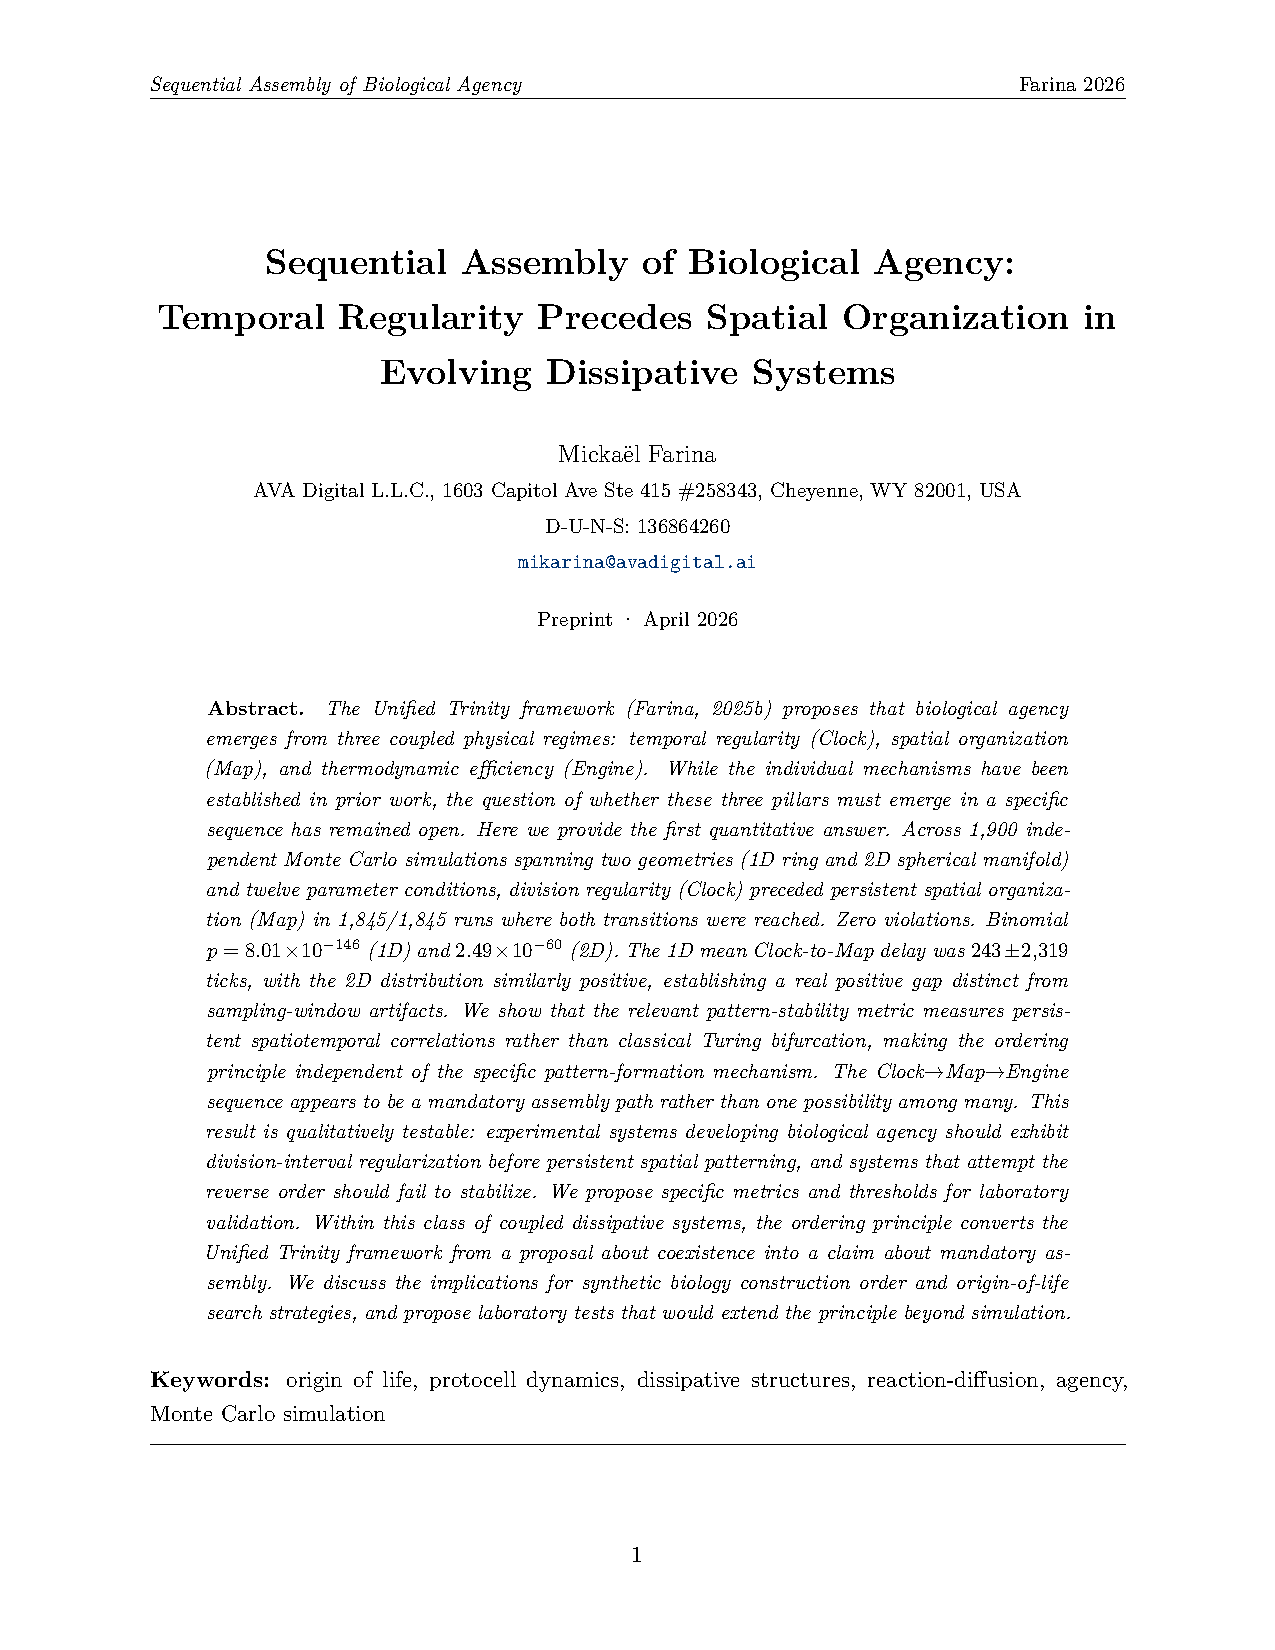
\includepdf[pages=-,pagecommand={\thispagestyle{stamp}},
            fitpaper=false,scale=0.94,offset=0 -22pt]
           {genesis_paper_farina_2026.pdf}

\end{document}
